\documentclass[12pt]{article}


\usepackage[utf8]{inputenc} % allow utf-8 input
\usepackage[T1]{fontenc}    % use 8-bit T1 fonts
\usepackage{hyperref}       % hyperlinks
\usepackage{url}            % simple URL typesetting
\usepackage{booktabs}       % professional-quality tables
\usepackage{amsfonts}       % blackboard math symbols
\usepackage{nicefrac}       % compact symbols for 1/2, etc.
\usepackage{microtype}      % microtypography




\usepackage[style=numeric,backend=bibtex,maxbibnames=99]{biblatex}
\addbibresource{references.bib}

\usepackage{graphicx}
\usepackage{caption}
\usepackage{subcaption}
\usepackage{float}
\usepackage{amsmath,amsfonts,amsthm,bm} % Math packages

\graphicspath{{img/}} %Setting the graphicspath
\usepackage{titling}

\setlength{\droptitle}{-10em}
%opening
\title{Removing Noise from Speech with Deep Learning\\
	\Large{First Milestone}}
\author{}
\date{}

\begin{document}
	% \nipsfinalcopy is no longer used
	
	\maketitle
	\section{Task summary}
	Our goal is to reduce (or in the best case, entirely remove) the noise from audio recordings containing noisy speech. The idea is to use the WaveNet\cite{wavenet}\cite{rethage2018wavenet} architecture to generate clean audio from the noisy one.
	
	
	\section{Data acquisition and exploration}
	For our training and testing data, we used a dataset called "\href{https://datashare.is.ed.ac.uk/handle/10283/2791}{Noisy speech database for training speech enhancement algorithms and TTS models}"\cite{dataset} by the University of Edinburgh. It consists of $\sim$23000 clean-noisy pairs from 56 different speakers. 
	The samples are stored in separate .wav files of varying length.  
	
	\begin{figure}[H]
		\centering
		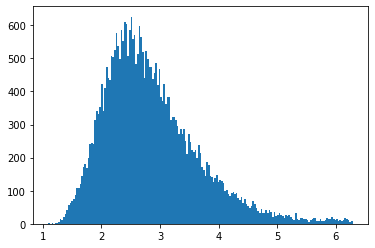
\includegraphics[width=.5\linewidth]{durations}
		\caption{Duration distribution histogram of a subset of speeches}
	\end{figure}
	
	
	
	\section{Data preprocessing}
	\subsection{Data selection by duration} \label{sel_dur}
	We intend to zero pad the data in order to make the samples the same length. To reduce the number of zeroes, we only use the $n$ samples that are closest to each other in duration. This way, we decrease the number of training samples, but hopefully, the efficiency of our network will be much better.
	
	\subsection{Zero padding} \label{pad}
	Our network architecture only supports samples of the same length. To fulfill this constraint, we add zeroes to the end of each recording. The number of necessary zeroes is calculated from the difference between the longest and the current sample.
	
	
	\begin{figure}[H]
		\centering
		\begin{subfigure}{.5\textwidth}
			\centering
			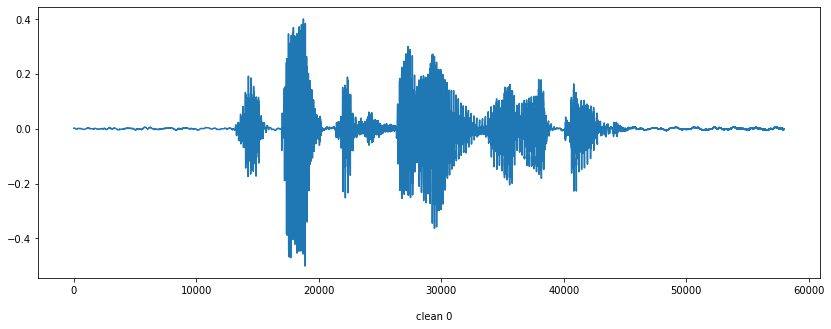
\includegraphics[width=.8\linewidth]{wave_clean}
			\caption{clean}
			\label{fig:wave_clean}
		\end{subfigure}%
		\begin{subfigure}{.5\textwidth}
			\centering
			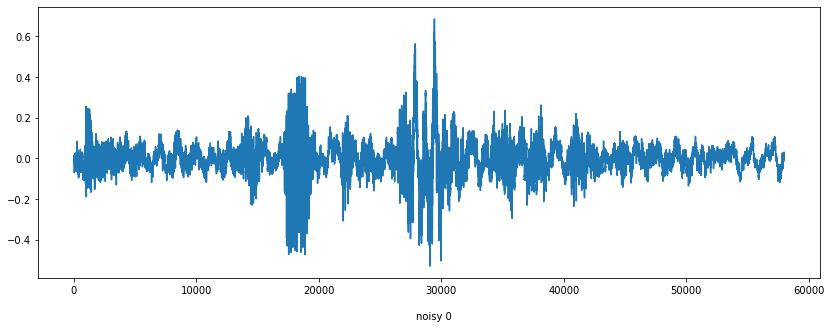
\includegraphics[width=.8\linewidth]{wave_noisy}
			\caption{noisy}
			\label{fig:wave_noisy}
		\end{subfigure}
		\caption{An example clean-noisy pair}
		\label{fig:clean_noisy}
		
		\begin{subfigure}{.5\textwidth}
			\centering
			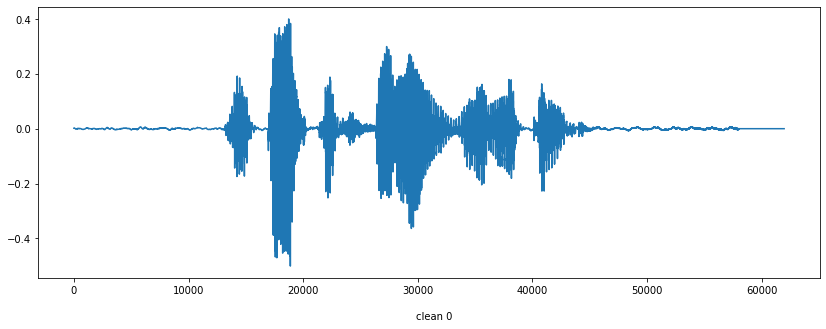
\includegraphics[width=.8\linewidth]{wave_clean_padded}
			\caption{clean}
			\label{fig:wave_clean_padded}
		\end{subfigure}%
		\begin{subfigure}{.5\textwidth}
			\centering
			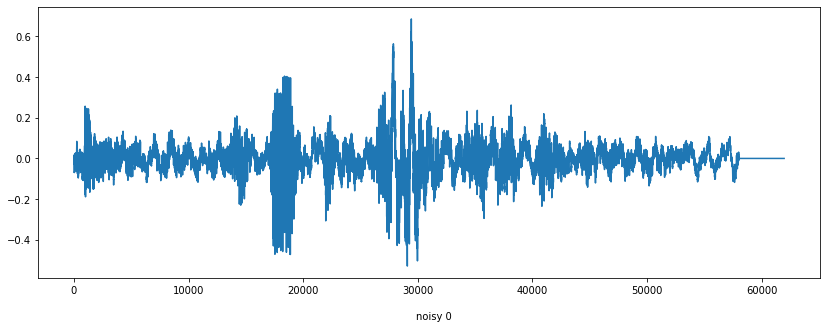
\includegraphics[width=.8\linewidth]{wave_noisy_padded}
			\caption{noisy}
			\label{fig:wave_noisy_padded}
		\end{subfigure}
		\caption{An example clean-noisy pair after zero padding}
		\label{fig:clean_noisy_padded}
	\end{figure}

	\subsection{\boldmath$\mu$-law transformation} \label{mulaw}
	To make future computations faster we, reduce the samples to 8 bit with $\mu$-law transformation.
	
	\begin{figure}[H]
		\centering
		\begin{subfigure}{.5\textwidth}
			\centering
			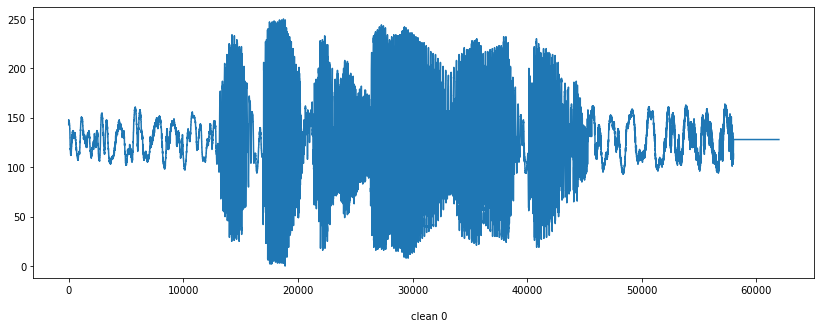
\includegraphics[width=.8\linewidth]{wave_clean_padded_mulaw}
			\caption{clean}
			\label{fig:wave_clean_padded_mulaw}
		\end{subfigure}%
		\begin{subfigure}{.5\textwidth}
			\centering
			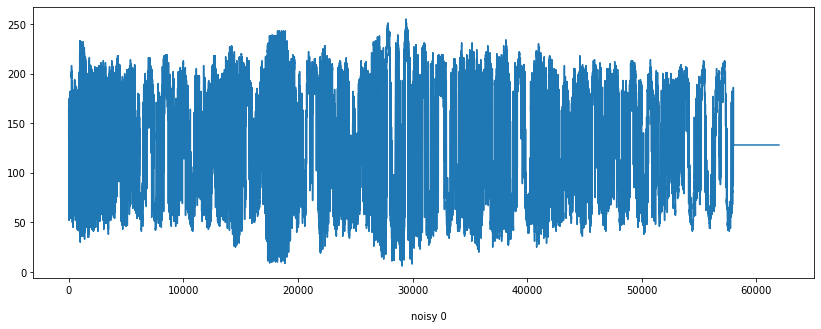
\includegraphics[width=.8\linewidth]{wave_noisy_padded_mulaw}
			\caption{noisy}
			\label{fig:wave_noisy_padded_mulaw}
		\end{subfigure}
		\caption{An example clean-noisy pair after padding and $\mu$-law transformation}
		\label{fig:clean_noisy_padded_mulaw}
	\end{figure}
	
	
	
	\subsection{Other preprocessing approaches}
	
	The techniques mentioned above are the preprocessing steps we are using right now. Because we don't have a model yet, we can't be sure if these are the right steps, so we came up with other approaches if we find out that the original data manipulation is not suitable for our network. These steps are shown in the figure\textsubscript{\ref{fig:DataToModelPic}} below.
	
	\begin{figure}[H]
	\centering

		\centering
		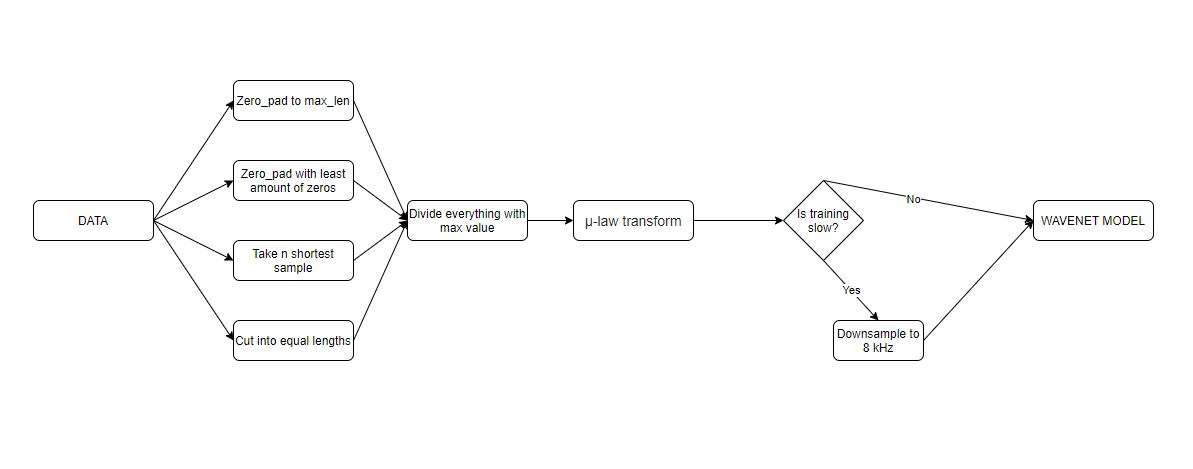
\includegraphics[width=1\linewidth]{DataToModelPic}
		\caption{Preprocessing flowchart}
		\label{fig:DataToModelPic}
	\end{figure}
	\subsubsection{Making the samples the same length}
	\begin{itemize}
		\item \textbf{Zero padding to maximum length}
		
		This approach is the easiest to implement. We find the longest sample and zero pad the others to match its length (so we can use all the audio from the training set).
		The problem with this approach is that the number of zeroes added to some of the shorter samples is a lot compared to their original size, and we don't know how well our model can handle it. The increase in size means that we will need a vast amount of memory to store it.
		The other disadvantage is that if the model can handle the changes, the learning will probably be much slower than before because of the unnecessary zeroes.
		
		\item \textbf{Zero padding with the least amount of zeroes}
		
		This step is what we described in sections \ref{sel_dur} and \ref{pad}.
		
		\item \textbf{Take the $n$ shortest samples}
		
		In this approach, we select an arbitrary number of samples from the beginning of our dataset (the data is arranged from short to long). This way, the number of zeroes in the padding is small, and the memory requirement is reduced drastically. Because of the reduction in the number of samples, the learning will be faster, but finding enough test data with the necessary length could be challenging.
		
		\item \textbf{Cut the samples into equal lengths}
		
		For this technique, we have to find the optimal sample length (which could be hard) and discard every data point shorter than that. After we figured out the optimal length, we cut the end of all longer samples to match that length. This process could provide us optimal sized data, but cutting can break the cohesion of the audio.
		
		
		
	\end{itemize}
	\subsubsection{Divide everything with max value}
	The $\mu$-law transform we described in section \ref{mulaw} needs inputs between -1.0 and 1.0. Dividing every value with the maximum solves this problem.
	
	\subsubsection{Downsampling to 8kHz}
	
	If we figured out the right combination of preprocessing steps, and the only problem is the speed of training, we will downsample the audio to 8kHz. This step can make training much faster. On the other hand, the quality of the audio will be worse.
	
	\newpage
	\printbibliography
	
	
\end{document}
